\documentclass[11pt,a4paper]{article}
\usepackage[margin=25mm]{geometry}
\usepackage[T1]{fontenc}
\usepackage[utf8]{inputenc}
\usepackage[british]{babel}
\usepackage{lmodern,microtype,amsmath,amssymb,amsthm,booktabs,tabularx,graphicx}
\usepackage{xcolor,caption,placeins,tikz,listings}
\usetikzlibrary{arrows.meta,positioning}
\definecolor{ink}{HTML}{243340}
\definecolor{figteal}{HTML}{007F86}
\definecolor{warm}{HTML}{C86428}
\definecolor{pale}{HTML}{D8EEF0}
\definecolor{light}{HTML}{F2F5F7}
\usepackage[colorlinks=true,linkcolor=figteal,citecolor=figteal,urlcolor=figteal]{hyperref}
\hypersetup{pdftitle={Direct Boolean Index Schemata for Scheduling and Scratch Allocation},pdfauthor={Alberto Hernandez-Espinosa}}
\captionsetup{font=small,labelfont=bf}
\setlength{\parskip}{4pt}
\setlength{\parindent}{0pt}
\setlength{\emergencystretch}{2em}
\graphicspath{{generated/}}
\lstset{basicstyle=\ttfamily\footnotesize,backgroundcolor=\color{light},breaklines=true,columns=fullflexible,keepspaces=true,showstringspaces=false}
\newtheorem{proposition}{Proposition}
\newcommand{\bits}{\{0,1\}}
\newcommand{\den}[1]{[\![#1]\!]}
\newcommand{\SAT}{\mathsf{SAT}}
\newcommand{\UNSAT}{\mathsf{UNSAT}}
\newcommand{\UNKNOWN}{\mathsf{UNKNOWN}}
\makeatletter
\newcommand{\tableinput}[1]{\@@input #1 }
\makeatother
\title{Direct Boolean Index Schemata for\\Scheduling and Scratch Allocation\\[5pt]\large A reproducible Luminal compiler case study}
\author{Alberto Hernandez-Espinosa}
\date{21 September 2026\\\small Research draft for internal review}

\begin{document}
\maketitle
\begin{abstract}
We study an executable compiler whose scheduling and scratch-allocation
decisions are witnesses of exact Boolean-set queries. Integer anchors and
free-coordinate masks represent families of candidate decisions; intersections,
differences and restrictions operate directly on these families. An independent
greedy construction supplies an incumbent, and bounded joint queries combine
legality with a strict cycle--scratch product target. We establish the elementary
algebra and construction invariants and evaluate a standalone implementation on
the pinned Luminal machine. On eight public programs, the combined score is
2.008466 relative to serial, versus 1.901379 for the frozen classical compiler.
The public gain already occurs in construction; joint optimization improves six
of 100 additional generated programs. Implementation refinements reduce full
compilation time by 2.1320 times relative to the previous direct version in the
final reviewed run, but compilation remains substantially slower than classical.
We report both outcomes, between-run variation, and representation limits.
Connections to Shannon decomposition, information bounds and Wolfram's account
of memory retrieval are separated by their actual role. The resulting artifact
is a basis for a controlled complexity study, not evidence of a general
complexity advantage.
\end{abstract}

\section{Question and contribution}
Can a compiler construct and improve a schedule by querying exact families of
Boolean decision indices, without first obtaining a schedule from a conventional
compiler? This case study answers that implementation question on a small,
precisely specified machine. The key operation is to intersect the set of legal
decisions with an objective threshold and retrieve a witness. Representing that
intersection can avoid enumerating individual assignments, when the predicates
admit useful structure.

The contributions are a direct integer-mask realization, an independently
constructed incumbent, bounded joint schedule/address queries, and a retained
evaluation with explicit correctness and evidence gates. Cube algebra and
constraint-based compilation have substantial prior art. Our contribution is
the particular construction and its measured behaviour, rather than a claim
that symbolic sets or integrated compilation are new.

Three costs must remain distinct throughout: the execution cycles of the
compiled program, its scratch footprint, and the time and memory used to compile
it. The direct method improves the aggregate public output score while spending
more compilation time. Even the output improvement is not uniform across
programs. An aggregate score cannot replace the component measurements.

\section{Machine and objective}
The experiment pins the Luminal interview repository at revision
\texttt{573b8a85}~\cite{luminal}; the bibliography gives the full identifier.
Inputs are straight-line operations in SSA dependency order, with consecutive
operation identifiers, static buffer ranges and supplied input cases. The
compiler must emit every operation exactly once. No instruction rewriting,
spilling or extra moves are allowed. Source arithmetic wraps modulo $2^{32}$;
schedule and address bookkeeping uses nonwrapping integers.

The scratchpad contains 256 words of 32 bits. Scalars occupy one word; vectors
occupy eight consecutive words at an address divisible by eight. Per-cycle issue
capacities are two for each of the load, scalar and vector engines, and one for
each of the store and flow engines. Latency controls result availability, not
how long an issue slot is reserved. If $i$ produces an argument of $j$,
\begin{equation}
 t_j\geq t_i+\ell_i.
\end{equation}
Overlapping memory accesses to the same buffer preserve source order when at
least one is a store: the later access issues at least one cycle after the
earlier. Two loads, or accesses to disjoint ranges, need no such ordering.

For a value $v$, let $b_v=t_{\operatorname{prod}(v)}+\ell_{\operatorname{prod}(v)}$
be its write cycle. Its lifetime is the \emph{inclusive} interval
\begin{equation}
 I_v=[b_v,e_v],\qquad
 e_v=\max\bigl(\{b_v\}\cup\{t_j:j\text{ consumes }v\}\bigr).
\end{equation}
An unused result still occupies its write cycle. Reuse requires strict temporal
separation because writes precede reads within a cycle. Scratch footprint $S$
is the largest allocated end address, including holes. Scored cycles $C$ are
the number of emitted bundles; they need not include the final completion cycle
of an unused result.

Let $(C_p^0,S_p^0)$ denote serial metrics for program $p$. For $m$ programs,
the official composite score is
\begin{equation}\label{eq:score}
 Q=\sqrt{\left(\prod_{p=1}^{m}\frac{C_p^0}{C_p}\right)^{1/m}
              \left(\prod_{p=1}^{m}\frac{S_p^0}{S_p}\right)^{1/m}}
   =\left(\prod_{p=1}^{m}\frac{C_p^0S_p^0}{C_pS_p}\right)^{1/(2m)}.
\end{equation}
For one fixed program, maximizing its score is equivalent to minimizing
$P=CS$. One component may worsen while the product improves. This is a declared
objective tradeoff, not a claim that memory reductions are execution speedups.
Only the eight visible programs are evaluated as the public challenge suite;
no private-grader result is available.

\section{Direct index schemata}
\subsection{Semantics and elementary algebra}
Use $n$ Boolean coordinates with least-significant-bit-first weights $2^i$.
Let $U=2^n-1$. A cube is $c=(n,a,f)$, with $a,f\in[0,U]$ and
$a\mathbin{\&}f=0$. Its anchor $a$ fixes the one bits and its mask $f$ marks
free coordinates. Its denotation is
\begin{equation}\label{eq:cube}
 \den{c}=\left\{a+\sum_{i:f_i=1}\epsilon_i2^i:
                         \epsilon_i\in\bits\right\}.
\end{equation}
The free-coordinate subset sums are the project's \emph{sumandos}. Freedom is
local to a schema; a free coordinate can represent a connected variable.
An index encodes an entire assignment of query fields. It is not itself a
physical scratch address, although one decoded field may be an address.
The broader project's \emph{index deconvolution} reconstructs an index family
from decimal anchors and their sumandos. Here, queries restrict those compact
families before decoding a witness. This is unrelated to inversion of a signal
convolution or to a physical memory operation.
For $n=0$, the denotation contains the empty assignment, index zero.

\begin{proposition}[Intersection, size and minimum]\label{prop:algebra}
For equal-width cubes $(n,a,f)$ and $(n,b,g)$, the intersection is empty exactly
when
\[
 (a\mathbin{\oplus}b)\mathbin{\&}\bigl(U\mathbin{\oplus}(f\mathbin{|}g)\bigr)
 \ne 0.
\]
Otherwise it is $(n,a\mathbin{|}b,f\mathbin{\&}g)$.
A cube has $2^{\operatorname{popcount}(f)}$ members and minimum member $a$.
The minimum of a nonempty finite cube union is the minimum of its anchors.
\end{proposition}
\begin{proof}
An assignment lies in both cubes precisely when it satisfies their fixed
coordinates. A conflict occurs at a coordinate fixed differently in both,
which is exactly the displayed mask test. In the compatible case a coordinate
is free in the intersection only if it is free in both; fixed ones are their
union. Each free coordinate has two independent choices, proving the size.
All free weights are positive and disjoint from the anchor, so their minimum
sum is zero. Taking the minimum over a union proves the last assertion.
\end{proof}

\begin{proposition}[Exact disjoint difference]\label{prop:difference}
Subtracting cube $d$ from cube $c$ produces an exact disjoint cover with at most
$n$ cubes when they intersect. If they do not intersect, the answer is $c$.
\end{proposition}
\begin{proof}
For an intersecting pair, consider coordinates free in $c$ but fixed in $d$,
in ascending order. At each coordinate emit the part opposite to $d$, and
continue with the matching part. Emitted parts have different first mismatches
and are disjoint. Every member of $c\setminus d$ has one such first mismatch;
the final matching part lies inside $d$ and is discarded. There are at most
$n$ split coordinates. With none, $c$ is contained in $d$ and the result is
empty.
\end{proof}
Restriction to a coordinate value is intersection with that coordinate's
literal cube. Integer intervals are decomposed into aligned binary blocks and
embedded in their fields, with all other coordinates free. Covers may overlap;
their sizes cannot in general be added to obtain union cardinality.

\begin{figure}[htbp]
\centering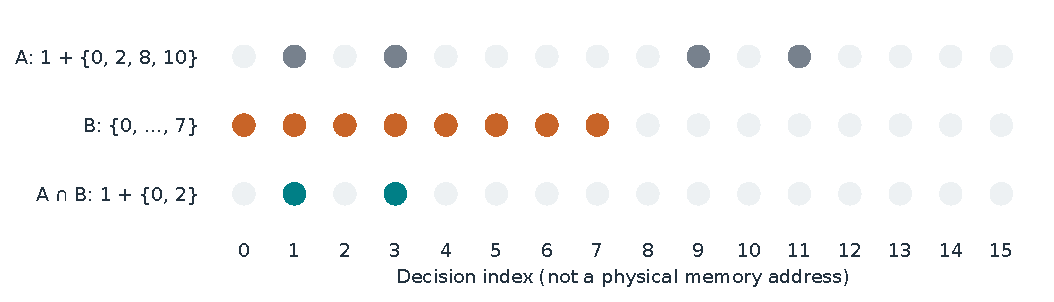
\includegraphics[width=\linewidth]{schema_example.pdf}
\caption{Exact four-coordinate example, with coordinate $i$ weighted by $2^i$.
Anchor 1 and free mask 10 denote $1+\{0,2,8,10\}$. Intersecting with indices
0 through 7 leaves $1+\{0,2\}$. The dots are a pedagogical expansion, not an
enumeration required by the implementation.}\label{fig:cube}
\end{figure}

\subsection{Queries and arithmetic}
A query is an AND/OR expression whose leaves are exact cube covers. The solver
maintains a current cube and pending predicates. AND adds requirements, OR
branches, and a leaf intersects each alternative with the current cube.
Alternatives have deterministic order. A depth-first traversal returns a cube
only after every required predicate is discharged. This avoids eagerly forming
the Cartesian product of all covers; it does not guarantee a small search.

\begin{proposition}[Query soundness and conditional completeness]
If leaves denote their predicates exactly, every returned accepting cube is
contained in the expression's denotation. If the finite search is exhausted
without a resource cutoff, absence of an accepting branch proves the expression
unsatisfiable in its declared universe.
\end{proposition}
\begin{proof}
Initially the current cube is the universe. Each leaf intersection preserves
exactly the assignments satisfying that leaf. AND requires all children and OR
enumerates their union. Induction over the pending expression and search
branches preserves these set identities. A completed branch therefore contains
only satisfying assignments. Exhausting all branches accounts for the whole
expression and proves emptiness if none accepts.
\end{proof}
The anchor of a returned cube is a witness; the first depth-first witness is
\emph{not} guaranteed to be the globally smallest index. Bootstrap explicitly
uses minimum anchors over complete feasible covers. A timeout or count cutoff
is $\UNKNOWN$, never $\UNSAT$. The latter refers only to the current domains
and fixed context, not all possible schedules.

Comparison leaves handle fields or constants with integer offsets. On a partial
cube, minimum and maximum operand values can settle an inequality for every
filling, or exclude every filling. An unresolved comparison splits the free bit
of greatest significance within either operand, breaking ties by highest
absolute coordinate; zero is explored first. Equality, disequality, constants
and identical fields are simplified exactly. All offsets are nonwrapping.
This is Boolean cofactoring: the identity
\begin{equation}\label{eq:shannon}
 F=(\neg x_i\wedge F|_{x_i=0})\vee(x_i\wedge F|_{x_i=1})
\end{equation}
underlies the partition, rather than a Shannon channel-capacity calculation.

\section{Compiler construction and bounded improvement}
\subsection{Independent bootstrap}
Let $H_0=\sum_i\ell_i$. Process operations in source order. For each, form a
time interval from its precedence lower bound to a safe upper bound below
$H_0$, subtract cycles with a full engine, and select the minimum feasible
index. The implementation tightens this upper bound using the number of blocked
cycles and the prefix latency sum; this preserves the earliest feasible cycle.
After scheduling, compute exact lifetimes. Allocate vectors before scalars and
sort each group by write cycle and producer ID. Exclude addresses colliding
with previously allocated values whose lifetimes overlap, then select the
minimum aligned address.

\begin{proposition}[Existence of the bootstrap choices]
For a legal nonempty input with positive latencies and total distinct-result
width at most 256 words, each scheduling and allocation choice exists,
provided query construction completes within its budget.
\end{proposition}
\begin{proof}
Write $h_i=\sum_{j<i}\ell_j$. Inductively $t_j\leq h_j$. Thus every data
predecessor is available by $h_i$, every ordered memory predecessor issues
before $h_i$, and no earlier operation issues at $h_i$. Consequently $h_i$ is
feasible and $h_i<H_0$. A minimum query cannot choose a later time.

For allocation, suppose $k$ vectors have already been placed. Inductively their
end addresses are at most $8k$, since each lowest-address choice could have
used the next fresh eight-word block. That block is therefore available for
the next vector regardless of temporal overlap. After all vectors, each scalar
could use the next fresh word. Reuse can reduce this high-water bound. Total
distinct-result width at most 256, guaranteed for the documented supplied
programs, therefore suffices. These are existence arguments, not claims of
optimal schedules or footprints.
\end{proof}

The policies are familiar greedy policies: earliest feasible cycle and lowest
legal address in a specified order. Their decisions are computed through schema
queries. No serial or classical schedule supplies the incumbent, and the direct
production path contains neither a BDD backend nor an external solver.
Failure during bootstrap emits no partial schedule and invokes no fallback.

\subsection{Joint legality and target queries}
Select at most four operations. Encode their issue times, produced-value
addresses and auxiliary engine lanes in contiguous LSB-first fields, ordered
by operation ID. Other decisions are fixed. Selected times lie within two cycles
of the incumbent and in $[0,\min(H_0,T)-1]$; selected addresses range over all
aligned starts ending at or below target memory $M$.

The query intersects domains and targets, data precedence, memory order, engine
capacity and scratch safety. Two selected or external operations sharing an
engine require different times or lanes. External lanes are fixed by operation
ID in each bundle. Since engine capacities are at most two, the pairwise rule
is equivalent to issue capacity after existentially quantifying selected lanes.
Lanes are not emitted machine instructions.

For every affected value pair $u,v$, scratch safety requires
\begin{equation}\label{eq:safety}
 a_u+w_u\leq a_v\ \vee\ a_v+w_v\leq a_u\ \vee\ e_u<b_v\ \vee\ e_v<b_u.
\end{equation}
The temporal comparison $e_u<b_v$ expands to $b_u<b_v$ and $t_j<b_v$ for
\emph{every} consumer $j$ of $u$, including consumers outside the window.
This exactly implements inclusive lifetimes. Fixed external decisions must
also satisfy $t_i<T$ and $a_v+w_v\leq M$; a violation makes the bounded query
infeasible. It does not silently expand the window.

For incumbent $(C,S)$ and $P=CS$, try target pairs
\begin{equation}
 (C-1,S),\quad (C,S-1),\quad
 \left(C+1,\left\lfloor\frac{P-1}{C+1}\right\rfloor\right),\quad
 \left(C-1,\min\left(256,\left\lfloor\frac{P-1}{C-1}\right\rfloor\right)\right).
\end{equation}
Remove undefined, duplicate and out-of-bound pairs, targets below dependency,
engine or result-width lower bounds, and any pair with $TM\geq P$.
Window priorities consider latest-issued operations and producers of the
highest scratch ends, followed by source-order windows of four advancing by
two, retaining the final shorter window. For a memory-reducing target, the
scratch window comes first. Windows are deduplicated deterministically.

\begin{figure}[htbp]
\centering
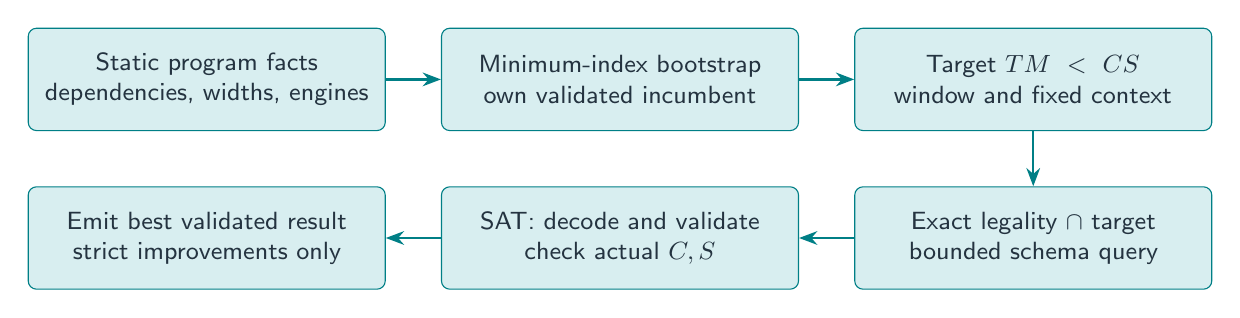
\begin{tikzpicture}[node distance=7mm,
 box/.style={draw=figteal,rounded corners=3pt,fill=pale,align=center,
 text width=43mm,minimum height=13mm,font=\sffamily\small,text=ink},
 arr/.style={-{Stealth},thick,draw=figteal}]
\node[box] (input) {Static program facts\\dependencies, widths, engines};
\node[box,right=of input] (boot) {Minimum-index bootstrap\\own validated incumbent};
\node[box,right=of boot] (target) {Target $TM<CS$\\window and fixed context};
\node[box,below=of target] (query) {Exact legality $\cap$ target\\bounded schema query};
\node[box,left=of query] (check) {SAT: decode and validate\\check actual $C,S$};
\node[box,left=of check] (output) {Emit best validated result\\strict improvements only};
\draw[arr] (input)--(boot);\draw[arr] (boot)--(target);
\draw[arr] (target)--(query);\draw[arr] (query)--(check);\draw[arr] (check)--(output);
\end{tikzpicture}
\caption{Production flow. UNSAT or UNKNOWN retains the incumbent and continues
within the remaining budgets. An accepted improvement restarts target selection.
A validator disagreement is recorded as a release-blocking discrepancy. The
classical and serial compilers are evaluation controls outside this flow.}
\end{figure}

\begin{lstlisting}[float=htbp,caption={Abstract optimizer loop; declarations above fix its search policy.}]
incumbent = independently_construct_and_validate(program)
while time_and_query_allowance_remain:
    improvement = false
    for target, window in deterministic_queries(incumbent):
        result = build_and_solve(legality AND target, shared_budget)
        if result is SAT:
            candidate = decode(result.cube.anchor)
            independently_validate_and_measure(candidate)
            record_discrepancy_if_invalid_or_target_breached()
            if valid AND within_target AND product_strictly_decreases:
                incumbent = candidate; improvement = true; restart
        # UNSAT and UNKNOWN preserve incumbent
    if not improvement: break
return incumbent
\end{lstlisting}

Internal validation checks structural machine legality. The evaluation harness
separately checks final memory for every supplied case of each measured output.
The optimizer measures actual cycles and footprint against the requested target;
passing machine validation alone is insufficient. Only strict product decreases
are accepted. Conditional on exact constraints and the independent checks,
legality is preserved and accepted objective values decrease. Neither property
proves global optimality. The test corpus checks the implementation; it is not
a formal proof of the full Python program or correctness on untested cases.

\subsection{Resource contract and implementation refinements}
The declared total soft allowance is 15 seconds, with at most 10 seconds for
optimization, 0.1 seconds per joint query and 32 attempted queries. Per-query
caps are 4,096 cubes per atomic cover, 50,000 visited cubes and 20,000 expression
records. Construction and search share a meter. One second of internal headroom
is reserved for final processing; the external isolated-process timeout is
20 seconds. Cooperative clock checks are not hard real-time guarantees.

The refined v4 implementation reduces repeated invariant checking inside proved
algebra operations, reuses exact relation covers within one compilation, avoids
repeated calendar reconstruction, and streamlines query accounting. Public cube
construction still validates inputs. Reuse is charged according to the declared
logical accounting; it does not increase the search allowance. Later repairs
restore clock checks before terminal verdicts and make the evidence checker
enforce its own frozen protocol. These optimizations target constant costs in
this implementation, not a different asymptotic problem.

\section{Evaluation design and evidence}
The primary dataset is the final independent lead run at reviewed revision
\texttt{1cf98da}, recorded on 20 September 2026. Production code is unchanged
from the preceding repair. The candidate export has 2,652 lines; its full hash
and that of frozen v3 are in Appendix~\ref{app:artifact}. Earlier runs are
retained to describe variability and repairs, not pooled as independent samples.

The fresh verifier passed 340 direct tests, the unchanged 11 public tests,
142 isolated programs with 277 cases, and eight CLI checks. The acceptance
corpus combines eight public programs, 30 historical regression programs, 100 generated inputs
and four stress inputs. Exact small-domain algebra/constraint tests,
independence checks and injected harness failures supplement output tests.
The official serial/classical/direct comparison retains all $8\times3\times3=72$
measurements and passes its seven release gates. The evidence audit passes 50
checks covering protocol, membership, hashes, measurement arithmetic and
verification artifacts.

For timing, five arms are measured: classical, frozen-v3 bootstrap, frozen-v3
full, candidate bootstrap and candidate full. Each public program has 15
repetitions, giving 600 rows. A separately frozen set of 100 additional
generator inputs has three repetitions in each arm, giving 1,500 rows.
The latter set uses different seeds but shares the development generator;
it is not an independent sample of real compiler workloads.

Each timed compilation uses a fresh process. Direct arms load only their
standalone export and pinned machine in an isolated directory. Arm order within
each program/repetition is seeded and shuffled. There are no warmups, excluded
outliers or silent retries. The compiler-call interval excludes import and
the harness's post-call correctness check. Internal validation performed by the
compiler remains inside its call time. Import time, total subprocess elapsed
time and process peak resident memory are separate measurements. Process
launch paths differ between classical and direct arms, so their process totals
also include different harness overheads.

For baseline $B$ and candidate $A$, the primary speedup statistic is
\begin{equation}\label{eq:timing}
 R=\exp\left[\frac1{8}\sum_{p=1}^{8}
       \log\frac{\operatorname{median}_r t_{B,p,r}}
                     {\operatorname{median}_r t_{A,p,r}}\right].
\end{equation}
The 95\% percentile intervals use 10,000 paired resamples of repetition
identifiers with seed 20260920. They condition on the programs and recorded run;
they quantify neither uncertainty over new programs nor between-run system
variation. A ratio of pooled medians is a different statistic and is explicitly
labelled wherever used.

The recorded environment is Python 3.13.7, macOS 26.6.2, arm64, with 28 logical
CPUs reported. The provenance does not identify the precise CPU model or control
thermal state. No verification or benchmark process launched by the lead ran
concurrently with these measurements. This does not imply complete system
quiescence.

\section{Results}
\subsection{Output quality and the optimizer ablation}
The public composite scores are serial 1.000000000, classical 1.901379121,
and direct 2.008466202. Both direct versions and both direct modes produce the
same public cycles and scratch metrics. The 5.6321\% composite advantage over
classical therefore belongs to bootstrap on this suite. It does not measure
the benefit of joint optimization, nor isolate representation from differing
greedy heuristics.

\begin{table}[htbp]\centering\small
\begin{tabular}{lrrrrrr}\toprule
&\multicolumn{2}{c}{Serial}&\multicolumn{2}{c}{Classical}&\multicolumn{2}{c}{Direct, both modes}\\
Program&$C$&$S$&$C$&$S$&$C$&$S$\\\midrule
\tableinput{generated/quality_rows.tex}
\bottomrule\end{tabular}
\caption{Exact public output metrics from retained measurements. $C$ is emitted
cycles and $S$ is scratch words. Direct is worse on both components for
\texttt{mixed\_broadcast}; the aggregate gain is not universal.}\label{tab:quality}
\end{table}

\begin{figure}[htbp]\centering
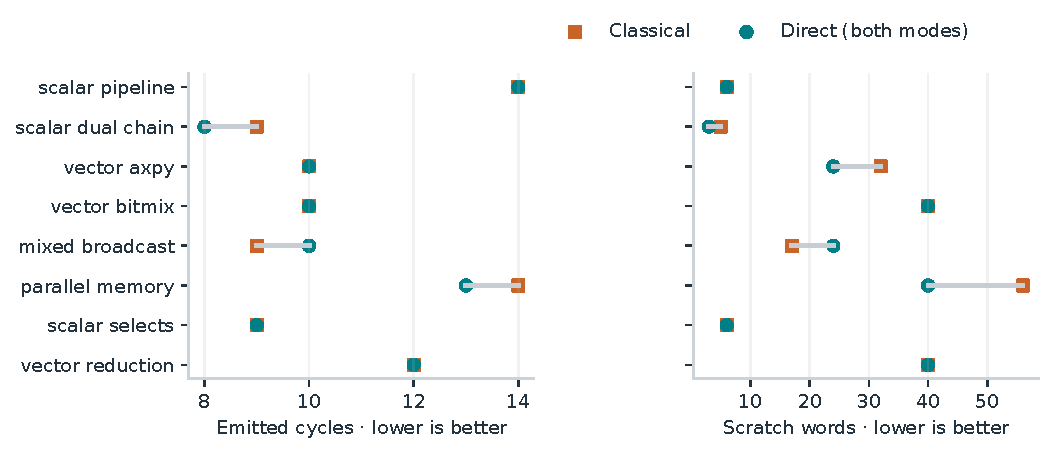
\includegraphics[width=\linewidth]{output_quality.pdf}
\caption{Component differences against classical. Coincident markers indicate
equal metrics. The two axes have different units; neither is compiler runtime.}
\end{figure}

On the 100 additional programs, score geomeans relative to serial are
2.370890261 for classical, 2.362098438 for bootstrap and 2.376596963 for full
direct compilation. Six distinct programs improve through joint optimization;
18 accepted improvements are recorded across three repetitions, not 18
independent improved programs. Candidate and frozen direct metrics agree on
every public and generated timing row. Bootstrap is slightly below classical
on this generated aggregate, while full is slightly above it. The public ordering
therefore does not transfer unchanged even to this related generator.

\begin{figure}[htbp]\centering
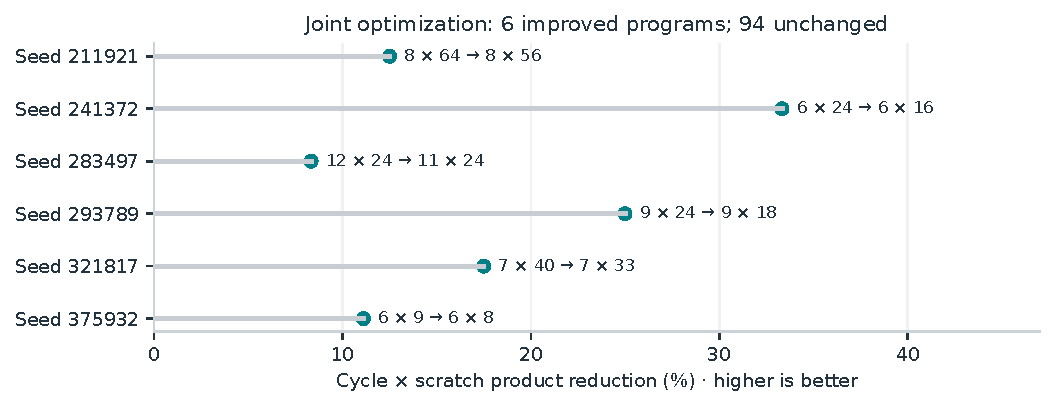
\includegraphics[width=\linewidth]{optimizer_ablation.pdf}
\caption{The six additional programs improved by joint optimization, with
$(C\times S)$ before and after. The other 94 programs have zero product change.
Each pair of metrics repeats in all three measurements, for both direct
versions. This is an optimizer-on/off comparison within the direct compiler.}
\end{figure}

\subsection{Compilation time and memory}
In the final reviewed run, full-direct compilation is 2.132005693 times faster
than frozen v3 by Equation~\ref{eq:timing}, with interval
[2.126779601, 2.137538179]. Bootstrap is 1.162943978 times faster, with interval
[1.147124692, 1.168961407]. The full 2.00-times engineering target is met in
this run; the bootstrap 1.20-times target is missed. These targets were declared
before measurement and are separate from mandatory correctness gates.

\begin{figure}[htbp]\centering
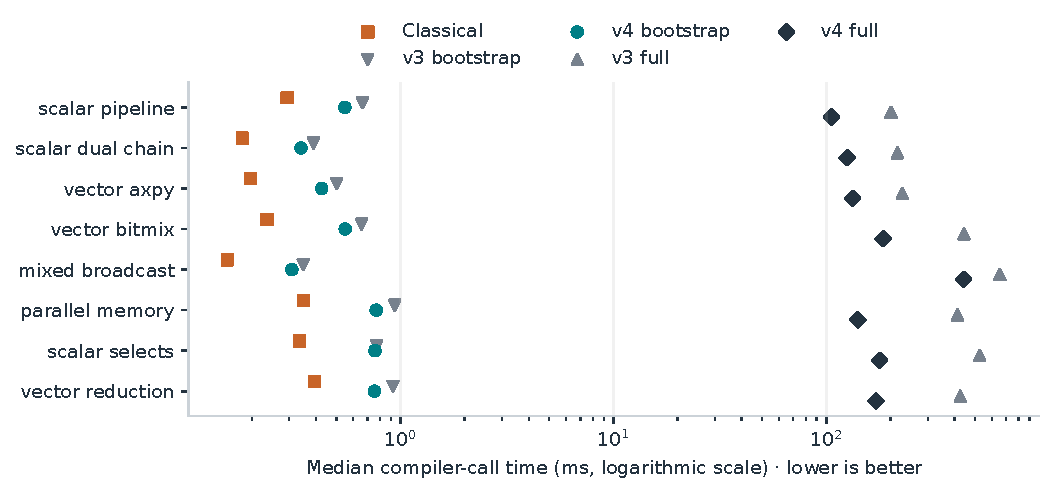
\includegraphics[width=\linewidth]{compile_times.pdf}
\caption{Median compiler-call times from 15 repetitions per public program.
The logarithmic axis keeps the classical/direct gap visible alongside the v3/v4
improvements. Bootstrap and full compilation have identical public output
quality despite their different costs.}\label{fig:times}
\end{figure}

Direct compilation remains slower than classical. The geometric means of
per-program median \emph{candidate/classical} ratios are 2.0696 for bootstrap
and 657.5045 for full. Alternatively, the \emph{pooled} median call times are
0.26927 ms classical, 0.54962 ms bootstrap and 155.80323 ms full; dividing these
pooled medians gives about 2.04 and 578.61. Different aggregation explains the
different ratios; none supports classical-relative runtime superiority.

\begin{table}[htbp]\centering\small
\begin{tabular}{lrrrr}\toprule
Arm&Call (ms)&Import (ms)&Process (ms)&Peak RSS (MiB)\\\midrule
\tableinput{generated/resource_rows.tex}
\bottomrule\end{tabular}
\caption{Pooled medians across public timing rows. Peak RSS is whole-process
resident memory, including the interpreter and loaded modules; it is not
the cube representation size and is unrelated to the program's scratch words.
Each column is separately aggregated, so medians are not additive.}
\end{table}

\subsection{Variation and negative results}
The worker's last run, using the same production compiler, reported full
speedup 1.9471 and bootstrap speedup 1.1337. The lead's fresh run crosses the
full target, but does not erase the earlier miss or establish a reliably
achieved 2.00-times speedup. Figure~\ref{fig:variation} shows consecutive repaired
runs. Their within-run intervals are narrow compared with some between-run
changes. Two classical program medians changed substantially in earlier rounds;
the cause is not established. We therefore retain per-program values rather
than diagnosing the difference as hardware noise or attributing it to one edit.

\begin{figure}[htbp]\centering
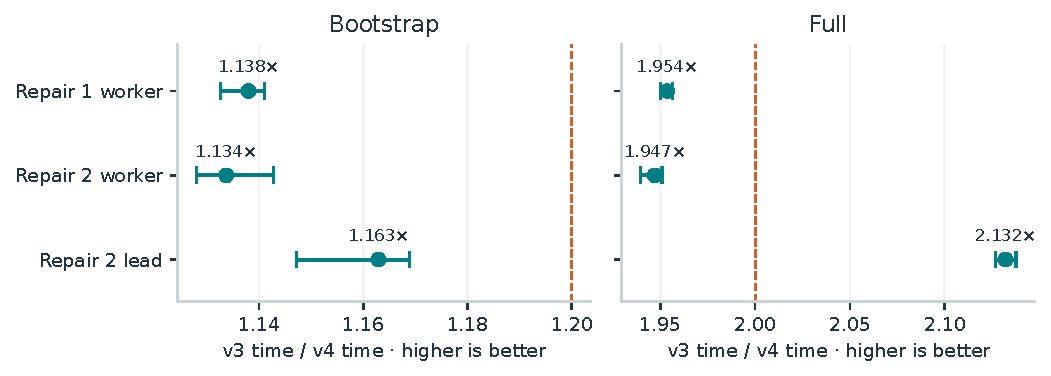
\includegraphics[width=\linewidth]{run_variability.pdf}
\caption{Three retained runs after production repairs. Dashed lines are the
original engineering targets. Error bars are paired within-run intervals;
they do not describe variation between runs. Production code is the same in
these three runs; evidence-checker changes distinguish the repair rounds.}
\label{fig:variation}
\end{figure}

The optimizer improves only a minority of generated inputs, adds no public
quality gain, and has substantial overhead. Bounded windows, target selection,
representation growth and search all constrain it; the per-query clock is not
the only limit. Count-limited queries can become faster even with unchanged
budgets. Prior attempts to infer a universal speedup ceiling from timeout
fractions are unsupported because queries can encounter different kinds of
limits after optimization. No measured slowdown here proves that the method
can never beat a particular classical implementation.

\section{Relation to prior ideas and complexity}
\subsection{Boolean covers and integrated compilation}
A cube is a conjunction of fixed literals; a flat cube cover is a disjunctive
normal form. Integer anchors change its storage and operations, not its
mathematical denotation. Bryant's ordered binary decision diagrams share
subfunctions in a graph and are canonical under a fixed variable order and
reduction rules~\cite{bryant}. This implementation instead uses direct masks
and factored AND/OR queries. Neither representation dominates all Boolean
functions; no BDD performance comparison is reported here.

Combining scheduling and allocation in one constraint model also has precedent.
Unison formulates integrated register allocation and instruction scheduling by
constraint programming and evaluates the resulting compiler on real target
architectures~\cite{unison}. Luminal's fixed scratch machine, restricted
transformations and four-operation neighborhoods define a much narrower study.
Neither its scores nor its times are comparable to Unison's published results.
The present measurements compare only the pinned local implementations.

\subsection{What is used from Shannon, and what is not}
Equation~\ref{eq:shannon} supplies the mathematical cofactor partition used by
Boolean splitting. Shannon's switching-circuit work is relevant historical
context~\cite{shannon49}. This identity does not bound the number of splits
needed to construct a useful accepting cover.

Two information questions must be distinguished. Shannon's communication
theory concerns source entropy and reliable communication under a specified
channel model~\cite{shannon48}. A finite memoryless source has entropy
$H(X)=-\sum_xp(x)\log_2p(x)$; a discrete memoryless channel has capacity
$\mathcal C=\max_{p(x)}I(X;Y)$. The Luminal compiler defines no noisy channel,
code rate or source distribution over its decision assignments. It therefore
does not implement or approach a measured Shannon communication limit.

Separately, there are $2^{2^n}$ subsets of an $n$-bit universe. A fixed-length
lossless description capable of distinguishing \emph{all} these subsets needs
at least $2^n$ bits in the worst case, by counting distinct codewords. For
variable-length descriptions, fewer than $2^n$ bits cannot describe all subsets
either, since there are only $2^{2^n}-1$ binary strings shorter than $2^n$.
This elementary counting argument concerns universal representation capacity,
not the running time of one compiler on a structured family. Storing large
families compactly is possible precisely because many families are structured.

\subsection{Wolfram's memory discussion}
Wolfram discusses exact retrieval by ordered lookup and hashing in his account
of human thinking, and suggests a possible connection to memory~\cite{wolfram}.
The useful motivation here is to ask what an indexed representation lets a
query recover without scanning all represented objects. The mechanism in this
compiler is exact logical restriction and witness extraction. It is not a model
of human memory, cellular-automaton hashing or approximate associative recall.
Ordinary implementation caches and provenance hashes do not establish such a
connection. The conceptual influence belongs in the research motivation, while
claims about computational behaviour must follow from the algorithms and data.

\subsection{An explicit representation limit}
\begin{proposition}[Parity needs an exponential flat cube cover]
For $n\geq1$, every exact cube-union representation of odd parity requires
$2^{n-1}$ singleton cubes.
\end{proposition}
\begin{proof}
Any cube with a free coordinate contains two assignments differing only in that
coordinate. They have opposite parity. Such a cube cannot be a subset of the
odd-parity set. In an exact union, each cube must be a subset, since a union
cannot cancel an unwanted member. Every cube is therefore a singleton, and
there are $2^{n-1}$ odd-parity assignments.
\end{proof}

\begin{figure}[htbp]\centering
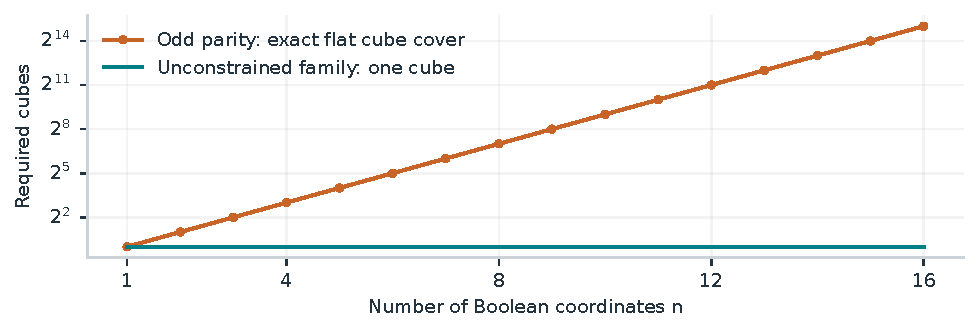
\includegraphics[width=.93\linewidth]{representation_limits.pdf}
\caption{Analytic representation examples, not compiler scaling measurements.
An unconstrained family is one cube; an exact flat cover of odd parity needs
exponentially many. This lower bound is specific to flat cube unions and does
not prove the same growth for factored expressions or decision diagrams.}
\end{figure}

A cube with $k$ free coordinates describes $2^k$ indices using two $n$-bit
masks, apart from metadata. This is a representation saving, not $2^k$ answers
computed at constant total cost. Expanding those members takes at least their
output size. For arbitrary $n$, Python integer operations themselves scale
with the number of machine words; treating an unbounded integer as a constant
cost object would hide complexity. Lazy factoring can avoid a large flat cover
on some predicates but does not imply tractable search in general. The parity
example also shows why the chosen representation must be named in every
compression claim.

\section{A reproducible starting point for a complexity study}
The artifact supports a precise next question: for which families of compiler
constraints do direct schemata reduce total construction and query cost?
Answering it requires families with controlled growth in operation count,
dependency width, field width, alias density and vector pressure. Report
expression size, cover sizes, bit widths, search visits, UNKNOWN rates,
compile time and process memory separately. Include preprocessing and cache
construction in the cost model.

Matched-heuristic implementations would isolate representation effects:
hold operation order, allocation order, windows, targets and budgets fixed,
and vary only the query backend. Stronger compiler baselines and different
generators address separate questions of competitiveness and generalization.
Repeat measurements across fresh runs and machines rather than treating repeated
timings of eight programs as independent workloads. Adversarial predicates,
including parity for flat covers, should accompany cases designed to compress.

No such scaling experiment is claimed in this draft. The present evidence
supports exact structured operations, validated bounded optimization and a
measured quality/cost tradeoff. It does not establish global optimality,
polynomial worst-case complexity, universal compression, or a separation of
complexity classes. The combination of positive and negative results makes the
compiler useful as an instrument for those more narrowly specified experiments.

\appendix
\section{Artifact and reproduction}\label{app:artifact}
The paper directory contains the editable manuscript, figure generator,
generated PDF/PNG figures, tables and an input hash manifest. All numerical
figures are derived from retained evidence; the set and parity figures are
labelled mathematical illustrations. No benchmark was rerun to select a better
paper result. The primary evidence root, relative to \texttt{luminal-challenge}, is
\begin{lstlisting}
results/direct_index_v4_optimization_repair2/lead_review/
\end{lstlisting}
The authoritative files are \path{final/runs.json},
\path{final/provenance.json}, \path{verification/summary.json},
\path{comparison/runs.json} and \path{measurement_audit.json}.
The frozen-v3 export and evaluation corpus are under
\texttt{results/direct\_index\_v4\_optimization/baseline/}.
The candidate and frozen export SHA256 digests, respectively, are
\begin{lstlisting}
d14bf39b450aaa5fe73c41a3236980e219089e527ae43007781d78e0059a5864
c0574395d339dae3b24e819955795c2a6165953c5966e46062c9bf9b18a50ce2
\end{lstlisting}
Figure generation checks current production hashes against retained provenance,
the candidate export, timing-row membership, component equality between
versions, and recomputed scores and speedups. The artifact README gives build
commands and validation results. To repeat the full empirical protocol, use new
output directories and the commands in the final lead review. Never overwrite
the historical measurement trees. The standalone compiler needs Python 3.10+
and the supplied machine module; plotting additionally uses NumPy and
Matplotlib, and the paper uses a standard pdf\LaTeX{} toolchain.

\clearpage
\section{Per-program compiler-call medians}
\begin{table}[htbp]\centering\small
\begin{tabular}{lrrrrr}\toprule
&Classical&v3 boot&v3 full&v4 boot&v4 full\\
Program&\multicolumn{5}{c}{Milliseconds, median of 15 calls}\\\midrule
\tableinput{generated/timing_rows.tex}
\bottomrule\end{tabular}
\caption{Unrounded raw timings are retained in the JSON evidence. These medians
underlie Equation~\ref{eq:timing} and Figure~\ref{fig:times}.}
\end{table}
\FloatBarrier

\section{Review status and assistance}
The implementation received local lead acceptance with limitations on
20 September 2026. That disposition covers the recorded compiler and evidence;
it is separate from manuscript peer review or a novelty determination.
The draft was prepared with Codex assistance; Claude Code assisted implementation
and repair work recorded in the repository. Checks include small-domain oracles,
independent machine execution, injected failures, source hashes, recomputation
of recorded measurements and inspection of primary literature. The author
retains responsibility for reviewing the proofs, claims and interpretation.

\clearpage
\begin{thebibliography}{9}
\raggedright
\bibitem{luminal} Luminal. \emph{Compiler challenge}, pinned source revision
573b8a85f4bdb8c3d8ba9f180d5f98dac875c902.
\url{https://github.com/luminal-ai/interview/tree/573b8a85f4bdb8c3d8ba9f180d5f98dac875c902}.
The retained reference files define the machine used here.
\bibitem{bryant} R. E. Bryant. Graph-based algorithms for Boolean function
manipulation. \emph{IEEE Transactions on Computers}, C-35(8):677--691, 1986.
\href{https://www.cs.cmu.edu/~bryant/pubdir/ieeetc86.pdf}{Author-hosted version}.
\bibitem{unison} R. Casta\~neda Lozano, M. Carlsson, G. Hjort Blindell and
C. Schulte. Combinatorial register allocation and instruction scheduling.
\emph{ACM Transactions on Programming Languages and Systems}, 2019.
\url{https://arxiv.org/abs/1804.02452}.
\bibitem{shannon49} C. E. Shannon. The synthesis of two-terminal switching
circuits. \emph{Bell System Technical Journal}, 28(1):59--98, 1949.
\href{https://deeplearning.cs.cmu.edu/S22/document/readings/Shannon49.pdf}{Primary paper}.
\bibitem{shannon48} C. E. Shannon. A mathematical theory of communication.
\emph{Bell System Technical Journal}, 27:379--423, 623--656, 1948.
\href{https://people.math.harvard.edu/~ctm/home/text/others/shannon/entropy/entropy.pdf}{Primary paper}.
\bibitem{wolfram} S. Wolfram. \emph{A New Kind of Science}. Wolfram Media,
2002. Chapter 10, Human Thinking, p.~622 (retrieval and hashing).
\url{https://www.wolframscience.com/nks/p622--human-thinking/}.
\end{thebibliography}
\end{document}
